\titleformat{\chapter}[display]
{\centering\LARGE\bfseries} % Formatting style
{\chaptername\ \thechapter} % Chapter label
{20pt} % Spacing
{\LARGE} % Title formatting

\chapter{Implementation, Testing and Results}

This chapter details the implementation and testing of the \emph{AI Content Factory}. It covers the configuration of the development environment, system integration practices, and provides a high-level description of the system's major modules. Additionally, this chapter outlines the comprehensive testing strategy applied to verify the correctness, reliability, and usability of the application, including Python-based white-box unit tests, integration tests, a detailed black-box testing matrix, and a usability analysis. The chapter closes by reporting the quantitative and qualitative results obtained from the completed system, together with an explicit statement of the limitations that bound them.

\section{Development Environment Setup}

Developing the AI Content Factory required configuring a modern asynchronous backend stack paired with a component-based frontend build system. The project setup is divided into backend, frontend, and environment configuration phases.

\subsection{Technology Stack and Packages}
The development libraries utilized in the application include:
\begin{itemize}
    \item \textbf{Backend Packages:} The backend dependencies were managed using Python virtual environments (\texttt{venv}) and installed via pip. Key packages include \texttt{fastapi} and \texttt{uvicorn} for web routing, \texttt{langgraph} for orchestrating stateful agents, \texttt{pydantic} for data validation, \texttt{openai} for GPT access, \texttt{google-genai} for native audio synthesis, \texttt{moviepy} for video rendering, and \texttt{deepeval} for academic grading.
    \item \textbf{Frontend Packages:} The frontend dependencies were managed using Node Package Manager (\texttt{npm}). They include \texttt{react} (v19) and \texttt{react-dom} for core UI construction, \texttt{vite} for high-speed local dev builds, \texttt{tailwindcss} for UI styling, and \texttt{lucide-react} for standard dashboard icons.
\end{itemize}

\subsection{Repository Setup and Version Control}
The system repository was initialized using Git and hosted on GitHub to enable audit trails and modular work. We used standard branching models:
\begin{itemize}
    \item The \texttt{main} branch represents stable, deployment-ready code.
    \item Feature branches (e.g., \texttt{feature/langgraph-checkpoints}, \texttt{feature/gemini-audio}) were merged into `main` only after passing local validation scripts.
    \item Environment variables were managed using a local `.env` configuration file to prevent accidental pushes of API keys to the remote repository.
\end{itemize}

\section{System Integration}

System integration refers to the process of binding the backend agent graph to the frontend dashboard and persisting data across client-server cycles. The integration process is structured around two key communication channels:

\begin{enumerate}
    \item \textbf{Asynchronous HTTP REST API:} Exposes endpoints for initiating content runs, uploading documents for semantic search, downloading completed markdown files, and playing rendered audio/video assets.
    \item \textbf{Real-Time WebSockets connection:} Connects the FastAPI backend to the React dashboard. During graph execution, agents write logging updates to a centralized `EventBus`. The EventBus translates these updates into JSON structures and streams them directly over WebSockets, allowing the user to view active agent thoughts in the Live Console.
    \item \textbf{Database State Checkpointing:} By binding the LangGraph engine to the SQLite database checkpointer, every graph state transition is stored. When the graph pauses for user approval at the Outline node, the FastAPI server serializes the state to the checkpointer and goes idle. When the user submits modifications, the API reloads the thread state from the database, merges changes, and resumes the execution thread.
\end{enumerate}

\section{High-Level Description of Major System Modules}

The codebase of the AI Content Factory is split into specialized modules, each implementing specific agent nodes:
\begin{itemize}
    \item \textbf{Topic Guard Module (\texttt{topic\_guard.py}):} Validates input queries, filters out inappropriate topics, and suggests corrections to ensure run quality.
    \item \textbf{Router Module (\texttt{routing.py}):} Analyzes the prompt and dynamically routes execution to Tavily search or closed-book writers.
    \item \textbf{Document Ingestion Module (\texttt{document\_ingest.py}):} Handles text extraction, semantic chunking, and similarity retrievals.
    \item \textbf{Orchestrator Module (\texttt{orchestrator.py}):} Generates the blog outlines and assigns evidence to sections.
    \item \textbf{Parallel Workers Module (\texttt{workers.py}):} Concurrently writes individual sections and merges them into a single markdown draft.
    \item \textbf{Quality Control Module (\texttt{quality\_control.py}):} Audits draft text against source files to detect hallucinations.
    \item \textbf{Revision Module (\texttt{revision.py}):} Modifies drafts based on quality control audit recommendations.
    \item \textbf{SEO Optimizer Module (\texttt{keyword\_optimizer.py}):} Integrates keywords naturally into the text.
    \item \textbf{Podcast Studio Module (\texttt{podcast\_studio.py}):} Calls the Google GenAI SDK to synthesize WAV podcasts.
    \item \textbf{Video Generator Module (\texttt{video.py}):} Searches Pexels, matches B-roll, and uses MoviePy to render subtitled MP4 videos.
    \item \textbf{Multimedia \& Image Decider Module (\texttt{multimedia.py}):} Plans image placements using detailed visual prompts and synthesizes high-resolution AI visuals via OpenAI (gpt-image-1 / DALL-E) and Pollinations AI (Flux engine).
    \item \textbf{Academic Judge Module (\texttt{evaluation.py}):} Calculates G-Eval scores using DeepEval and custom prompt rubrics.
\end{itemize}

\section{User Interface Implementation}

The user interface was built using Vite React, Vanilla CSS, and Tailwind CSS. The interface is styled with a modern dark theme to present a professional dashboard experience, with dynamic accent token inheritance for light theme mode (`data-theme="light"`). The core interactive components of the system are detailed below:

\begin{itemize}
    \item \textbf{Sidebar View \& Live Console Stream:} Lists all active and previous content generation runs, displaying their status (completed, running, paused, failed). It features a terminal window that displays WebSocket streams, printing colored logs in real-time as agents execute nodes. Additionally, it hosts theme-adaptive range sliders for section counts and image quantities. Figure \ref{fig:ui_dashboard} illustrates the main dashboard view.
    
    \begin{figure}[htbp]
        \centering
        \IfFileExists{Mian UI.png}{%
            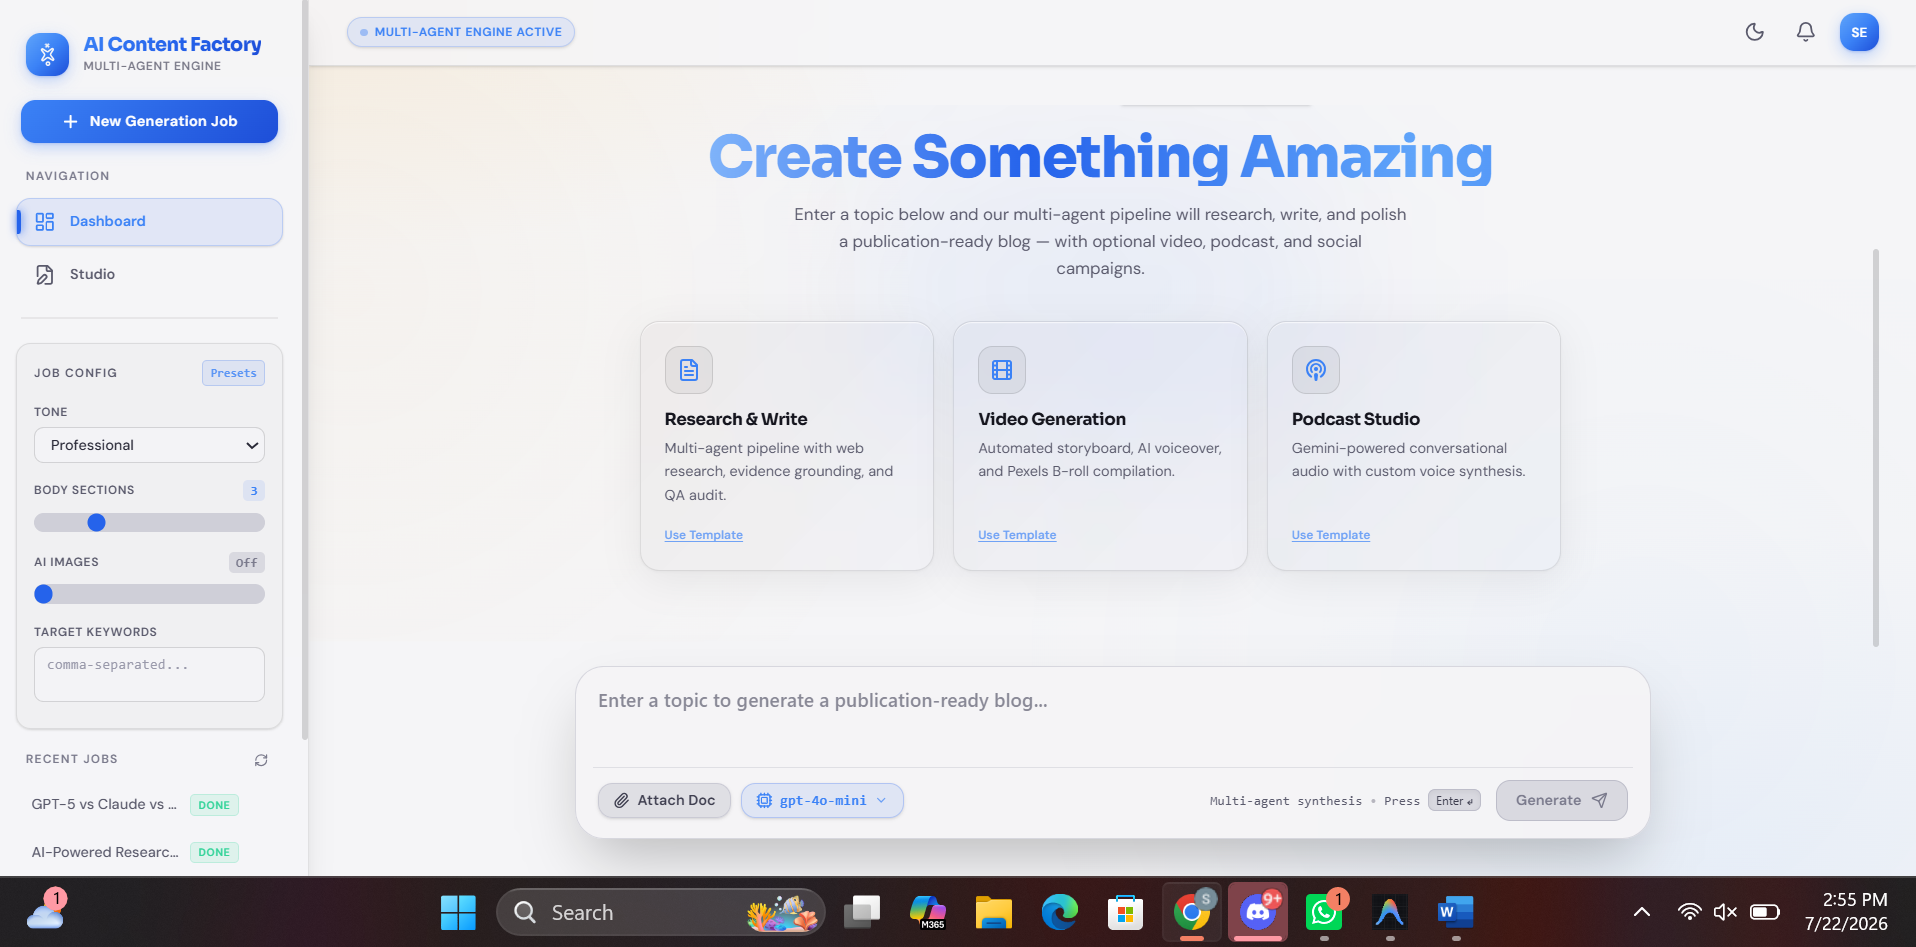
\includegraphics[width=0.9\textwidth,height=0.45\textheight,keepaspectratio]{Mian UI.png}%
        }{%
            \IfFileExists{dashboard_main.png}{%
                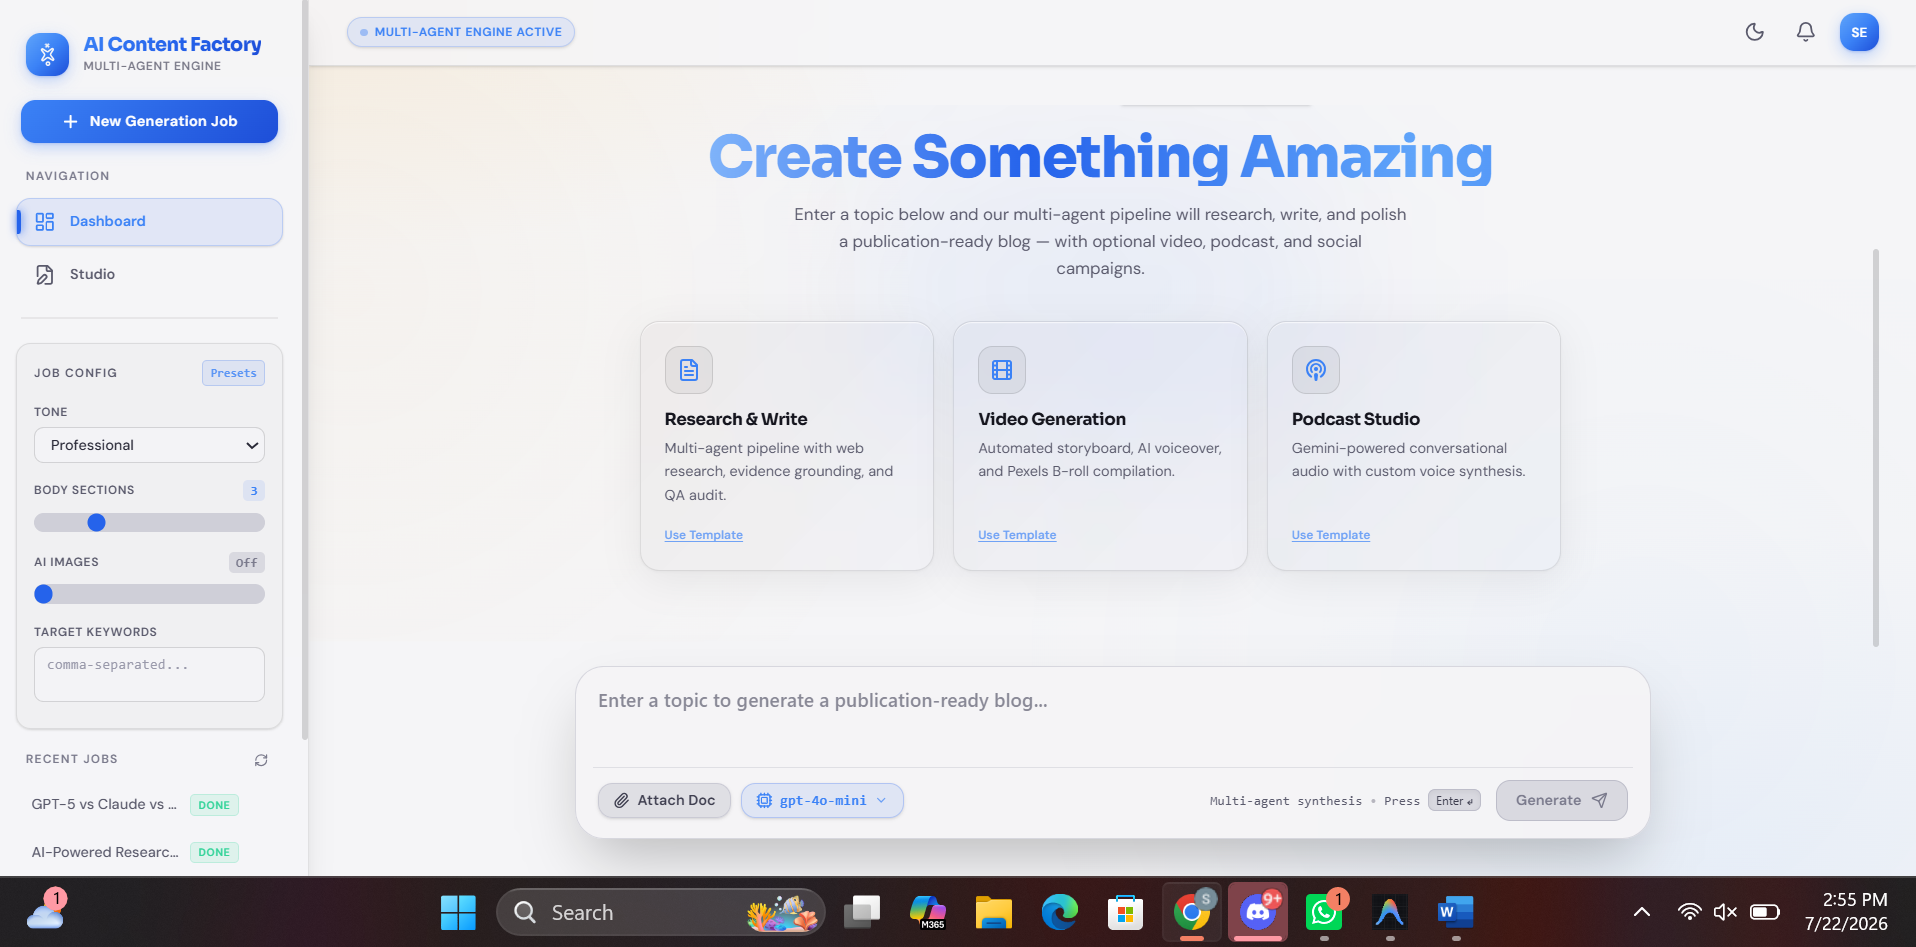
\includegraphics[width=0.9\textwidth,height=0.45\textheight,keepaspectratio]{dashboard_main.png}%
            }{%
                \framebox[0.9\textwidth]{\vbox to 5cm{\vfil\centering\textbf{[UI Screenshot Placeholder: Main Dashboard with Live Console]}\\\small(Save screenshot as `Mian UI.png` or `dashboard_main.png` in `BS_FYP_development` folder)\vfil}}%
            }%
        }
        \caption{AI Content Factory Main Dashboard with Live Console}
        \label{fig:ui_dashboard}
    \end{figure}

    \item \textbf{Interactive Plan Editor Drawer:} Opens when the backend hits the outline interrupt, showing a table of subheadings, word counts, and bullet points which the user can edit, reorder, or regenerate. Figure \ref{fig:ui_plan_editor} shows this Human-in-the-Loop review screen.
    
    \begin{figure}[htbp]
        \centering
        \IfFileExists{Plan editor.png}{%
            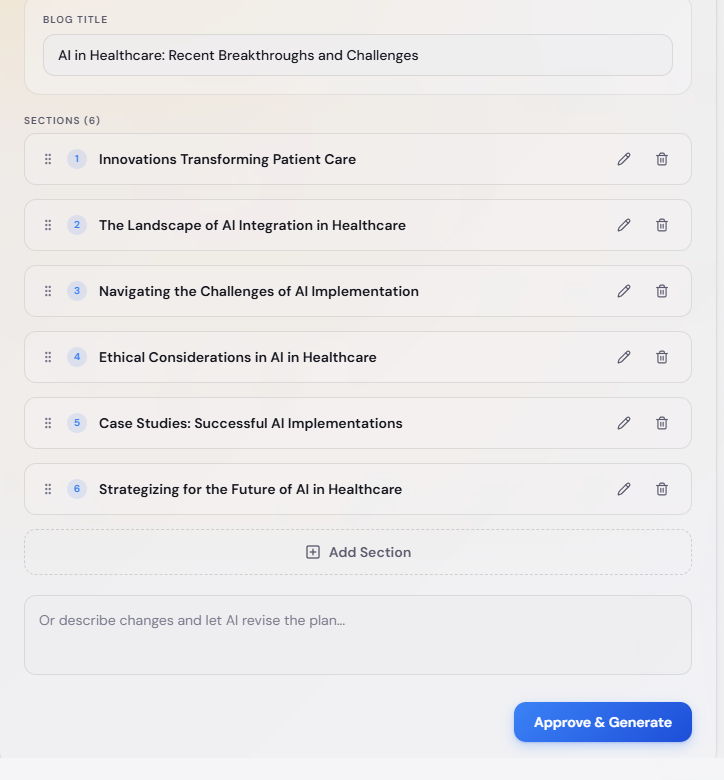
\includegraphics[width=0.9\textwidth,height=0.45\textheight,keepaspectratio]{Plan editor.png}%
        }{%
            \IfFileExists{plan_editor.png}{%
                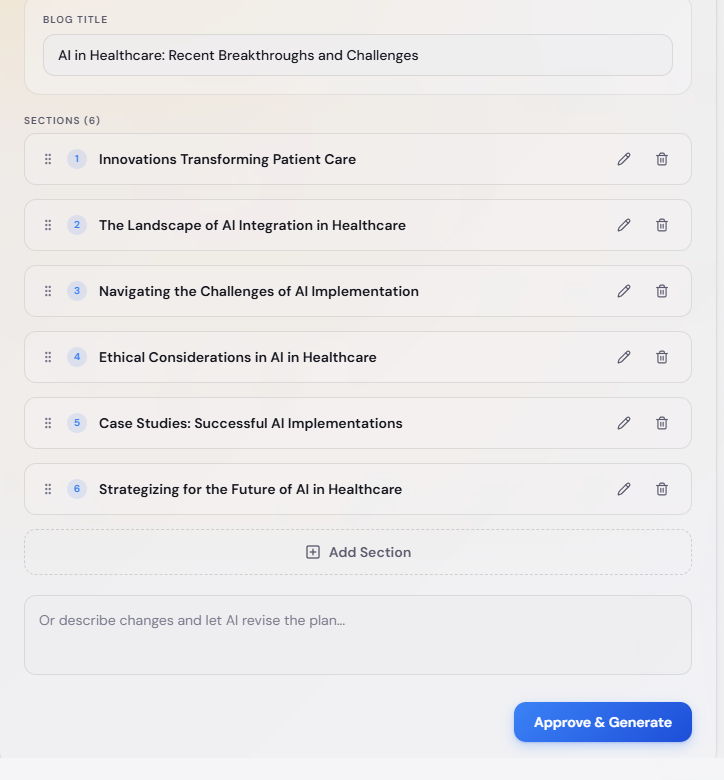
\includegraphics[width=0.9\textwidth,height=0.45\textheight,keepaspectratio]{plan_editor.png}%
            }{%
                \framebox[0.9\textwidth]{\vbox to 5cm{\vfil\centering\textbf{[UI Screenshot Placeholder: Interactive Plan Editor Drawer]}\\\small(Save screenshot as `Plan editor.png` or `plan_editor.png` in `BS_FYP_development` folder)\vfil}}%
            }%
        }
        \caption{Interactive Plan Editor and Outline Approval Drawer}
        \label{fig:ui_plan_editor}
    \end{figure}

    \item \textbf{Media Preview Windows \& Podcast Audio Player:} Integrates HTML5 video and audio players to play and preview synthesized WAV podcasts (generated natively via Gemini GenAI SDK) and MP4 videos, allowing users to verify audio narration quality and download generated media assets directly. Figure \ref{fig:ui_media_preview} displays the synthetic video preview player.

    \item \textbf{Agent Analytics \& Telemetry Dashboard:} Provides a centralized monitoring view for system performance, displaying real-time metrics including total estimated token consumption, API execution cost breakdowns, active worker node counts, section parallelization rates, and individual node execution latency statistics.

    \item \textbf{Quality Audit Scorecard:} Features an interactive DeepEval G-Eval Audit Scorecard panel displaying multi-dimensional quality metrics (Coherence, Relevance, Accuracy, Tone) and radar breakdown charts. Figure \ref{fig:ui_geval_scorecard} illustrates the DeepEval G-Eval audit scorecard, while Figure \ref{fig:ui_image_gallery} shows the Generated Images Gallery.
    
    \begin{figure}[htbp]
        \centering
        \IfFileExists{Media Preview.png}{%
            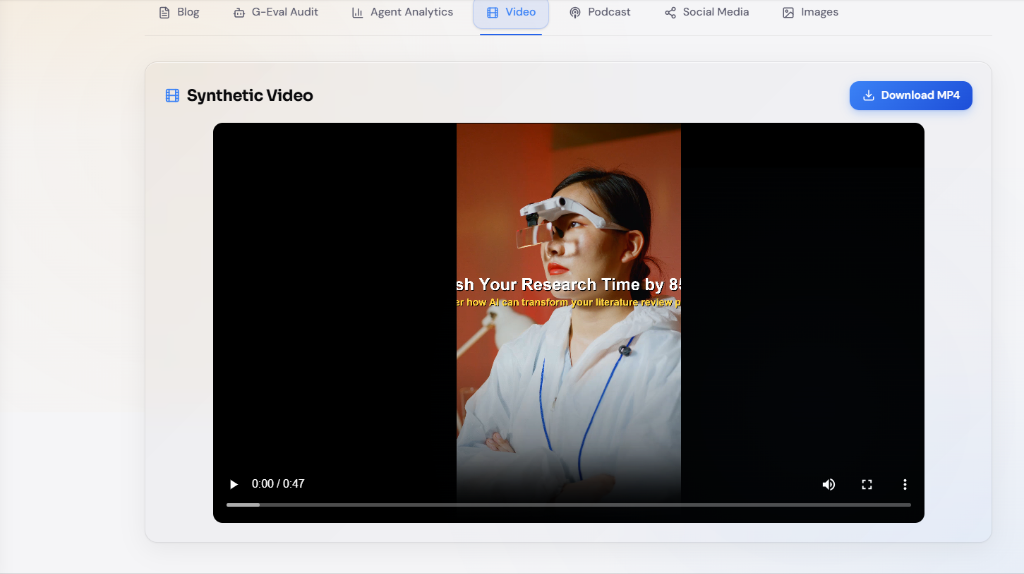
\includegraphics[width=0.9\textwidth,height=0.45\textheight,keepaspectratio]{Media Preview.png}%
        }{%
            \IfFileExists{media_preview.png}{%
                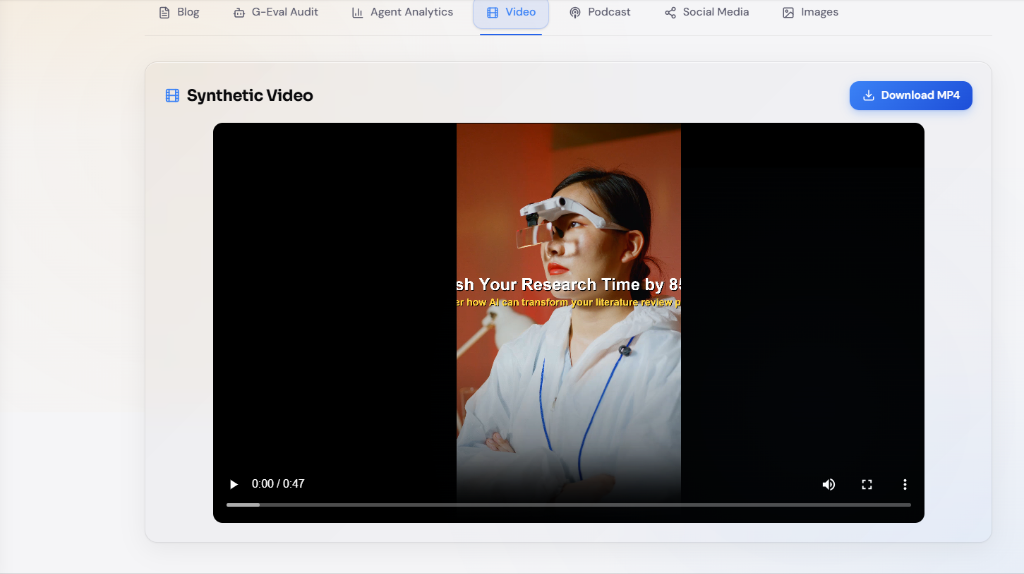
\includegraphics[width=0.9\textwidth,height=0.45\textheight,keepaspectratio]{media_preview.png}%
            }{%
                \framebox[0.9\textwidth]{\vbox to 5cm{\vfil\centering\textbf{[UI Screenshot Placeholder: Media Player Previews]}\\\small(Save screenshot as `Media Preview.png` or `media_preview.png` in `BS_FYP_development` folder)\vfil}}%
            }%
        }
        \caption{Synthetic Video Player and Media Preview Panel}
        \label{fig:ui_media_preview}
    \end{figure}

    \begin{figure}[htbp]
        \centering
        \IfFileExists{G-Eval Scorecard.png}{%
            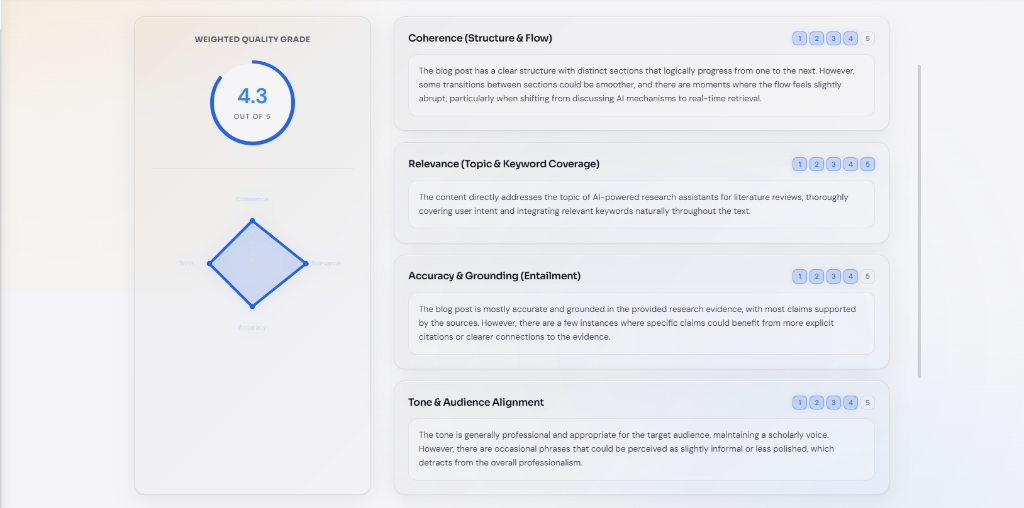
\includegraphics[width=0.9\textwidth,height=0.45\textheight,keepaspectratio]{G-Eval Scorecard.png}%
        }{%
            \IfFileExists{geval_scorecard.png}{%
                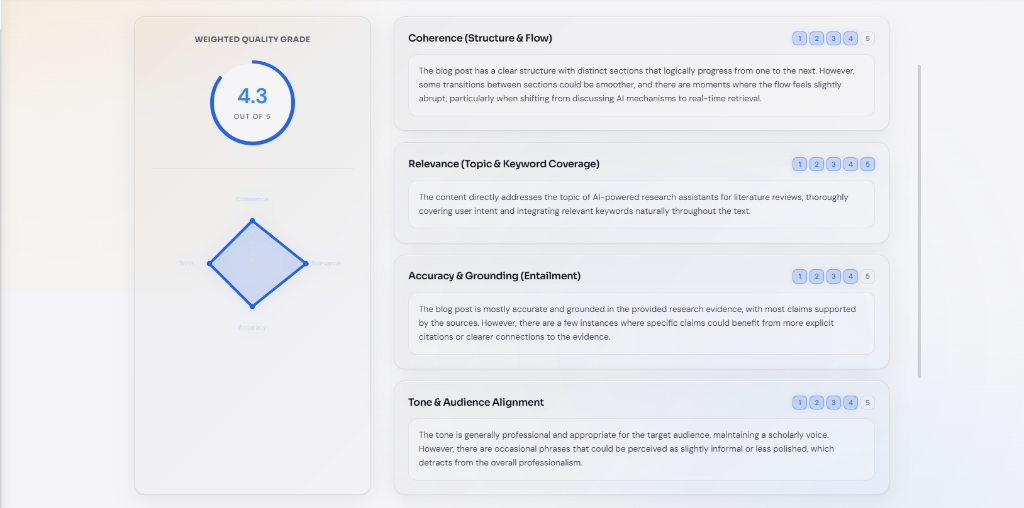
\includegraphics[width=0.9\textwidth,height=0.45\textheight,keepaspectratio]{geval_scorecard.png}%
            }{%
                \framebox[0.9\textwidth]{\vbox to 5cm{\vfil\centering\textbf{[UI Screenshot Placeholder: G-Eval Audit Scorecard]}\\\small(Save screenshot as `G-Eval Scorecard.png` or `geval_scorecard.png` in `BS_FYP_development` folder)\vfil}}%
            }%
        }
        \caption{DeepEval G-Eval Audit Scorecard and Multi-Dimensional Quality Metrics Panel}
        \label{fig:ui_geval_scorecard}
    \end{figure}

    \begin{figure}[htbp]
        \centering
        \IfFileExists{Image Gallery.png}{%
            
\includegraphics[width=0.9\textwidth,height=0.45\textheight,keepaspectratio]{Image Gallery.png}%
        }{%
            \IfFileExists{image_gallery.png}{%
                
\includegraphics[width=0.9\textwidth,height=0.45\textheight,keepaspectratio]{image_gallery.png}%
            }{%
                \framebox[0.9\textwidth]{\vbox to 5cm{\vfil\centering\textbf{[UI Screenshot Placeholder: Generated Images Gallery Grid]}\\\small(Save screenshot as `Image Gallery.png` or `image_gallery.png` in `BS_FYP_development` folder)\vfil}}%
            }%
        }
        \caption{Generated Images Gallery Grid and High-Resolution Visual Download Interface}
        \label{fig:ui_image_gallery}
    \end{figure}
\end{itemize}

\section{Testing}

To ensure the AI Content Factory operates reliably and generates high-quality content, we implemented a double-pronged testing strategy consisting of automated white-box tests and systematic black-box verification.

\subsection{White Box Testing}
White-box testing focuses on validating internal logic, data structures, and algorithms by inspecting the source code \cite{fowler_unit_test}. We wrote automated tests using Python's \textbf{pytest} framework.

\subsubsection{Unit Tests}
We created unit tests to verify individual functions and agent helpers. The
Topic Guard is a useful example because it is deliberately implemented as
\emph{two} tiers, and the unit tests document the boundary between them:

\begin{itemize}
    \item \texttt{\_trivial\_reject()} is a free, deterministic screen for
      \emph{malformed} input --- empty strings, topics under three characters
      or over two hundred, strings containing no letters, and keyboard
      gibberish. It runs first and costs nothing.
    \item \texttt{evaluate\_topic()} then calls the LLM guard, which judges
      whether a \emph{well-formed} topic is semantically unsafe.
\end{itemize}

Separating the two matters for cost: the overwhelming majority of rejected
submissions are malformed rather than harmful, and catching those without an
API call avoids spending tokens on input that was never going to produce a
blog post. The tests below (from \texttt{tests/test\_topic\_guard.py}) verify
the deterministic tier, including an explicit assertion that a well-formed but
unsafe topic is \emph{passed on} to the LLM tier rather than rejected here:

\begin{lstlisting}[language=Python]
from Graph.agents.topic_guard import _trivial_reject

def test_accepts_valid_topic():
    verdict = _trivial_reject("The Future of AI in Healthcare")
    assert verdict is None

def test_rejects_very_short_topic():
    verdict = _trivial_reject("Hi")
    assert verdict is not None
    assert verdict.is_safe is False

def test_rejects_gibberish():
    for topic in ("asdfgh", "aaaaaaaa", "lol"):
        verdict = _trivial_reject(topic)
        assert verdict is not None
        assert verdict.is_safe is False
        assert verdict.category == "nonsense"

def test_defers_semantic_safety_to_the_llm_guard():
    # A well-formed but unsafe topic must PASS the syntax screen: judging
    # harm requires semantics, so it is the LLM guard's responsibility.
    assert _trivial_reject("how to build a weapon") is None
\end{lstlisting}

\subsubsection{Integration Testing}
Integration testing verifies that multiple modules work together correctly. The
most important integration in this system is the one between LangGraph's
checkpointer and the Human-in-the-Loop interrupt, because it is what makes
crash recovery possible: the graph must persist its state at the interrupt,
report the correct next node, and resume from exactly that point on a second
invocation.

The test below (\texttt{tests/test\_checkpoint.py}) exercises that lifecycle
against a real \texttt{SqliteSaver} backed by an in-memory database. It uses a
minimal two-node graph rather than the full production graph deliberately: this
isolates the checkpointer contract from the behaviour of the fifteen agent
nodes, so a failure here is unambiguously a persistence fault rather than a
prompt or API problem. Note that resumption is triggered by passing
\texttt{None} as the input --- the signal to LangGraph that it should continue
from the stored checkpoint instead of starting a new run.

\begin{lstlisting}[language=Python]
import sqlite3
from typing import TypedDict
from langgraph.checkpoint.sqlite import SqliteSaver
from langgraph.graph import StateGraph, START, END

class SimpleState(TypedDict):
    count: int
    topic: str

def increment_node(state: SimpleState) -> dict:
    return {"count": state.get("count", 0) + 1}

def test_sqlite_saver_lifecycle():
    conn = sqlite3.connect(":memory:", check_same_thread=False)
    try:
        memory = SqliteSaver(conn)
        memory.setup()

        # The checkpointer must create its own persistence tables
        cursor = conn.cursor()
        cursor.execute("SELECT name FROM sqlite_master WHERE type='table'")
        tables = [row[0] for row in cursor.fetchall()]
        assert "checkpoints" in tables
        assert "writes" in tables

        workflow = StateGraph(SimpleState)
        workflow.add_node("step1", increment_node)
        workflow.add_node("step2", increment_node)
        workflow.add_edge(START, "step1")
        workflow.add_edge("step1", "step2")
        workflow.add_edge("step2", END)
        graph = workflow.compile(checkpointer=memory,
                                 interrupt_after=["step1"])

        # 1st run: executes step1, then halts at the interrupt
        thread_cfg = {"configurable": {"thread_id": "test_job_123"}}
        list(graph.stream({"count": 10, "topic": "AI Checkpointing"},
                          thread_cfg, stream_mode="values"))

        state = graph.get_state(thread_cfg)
        assert state.next == ("step2",)          # paused before step2
        assert state.values["count"] == 11       # step1's write persisted
        assert state.values["topic"] == "AI Checkpointing"

        # 2nd run: None as input resumes from the stored checkpoint
        list(graph.stream(None, thread_cfg, stream_mode="values"))

        final_state = graph.get_state(thread_cfg)
        assert final_state.next == ()            # reached END
        assert final_state.values["count"] == 12 # step2 ran exactly once
    finally:
        conn.close()
\end{lstlisting}

The production graph applies the same mechanism, compiling with
\texttt{interrupt\_after=["orchestrator"]} so that execution halts once the
outline has been planned and waits for the user's approval before dispatching
the parallel writing workers.

\subsection{Black Box Testing}
Black-box testing verifies that the system produces the correct output for a given input without inspecting internal code paths. We defined and executed several black-box test cases (Table \ref{tab:black_box_testing}).

\begin{table}[ht]
	\centering
	\renewcommand{\arraystretch}{1.3}
	\resizebox{1.09\textwidth}{!}{
	\begin{tabular}{|c|c|c|c|}
		\hline
		\textbf{Test Case ID} & \textbf{Input / Action} & \textbf{Expected Output} & \textbf{Result} \\
		\hline
		TC1 & User submits unsafe topic & Topic Guard flags topic and displays correction suggestions & Pass \\
		\hline
		TC2 & User uploads a PDF document & System parses PDF, generates embeddings, and retrieves relevant chunks & Pass \\
		\hline
		TC3 & Graph reaches Outline phase & System pauses execution, saves state, and opens Plan Editor Drawer & Pass \\
		\hline
		TC4 & User edits heading in UI and submits & Graph resumes execution, updates outline state, and routes to workers & Pass \\
		\hline
		TC5 & Reducer merges worker draft text & Quality Control auditor compares text against sources to flag hallucinations & Pass \\
		\hline
		TC6 & Quality Control finds inaccuracies & Graph routes draft to Revision agent for iterative corrections & Pass \\
		\hline
		TC7 & Podcast Studio node triggered & System calls Gemini API to synthesize conversational WAV audio & Pass \\
		\hline
		TC8 & Video Generator node triggered & System searches Pexels, matches B-roll, and renders subtitled MP4 video & Pass \\
		\hline
		TC9 & Evaluation node triggered & System generates Coherence, Relevance, Accuracy, and Tone scores & Pass \\
		\hline
		TC10 & User requests AI images & System generates 8k visual prompts via gpt-image-1/Flux and displays Gallery in UI & Pass \\
		\hline
	\end{tabular}
}
	\caption{Black-box testing results for the AI Content Factory}
	\label{tab:black_box_testing}
\end{table}

\subsection{Usability and User Test Report}
To evaluate the user experience, we conducted usability testing with five non-technical users. They were asked to create content, edit outlines, listen to podcasts, and watch rendered videos using the dashboard:
\begin{itemize}
    \item \textbf{Task Completion Rate:} 100\% of the users successfully created content and previewed the generated audio/video assets.
    \item \textbf{Usability Scores:} Users rated the system on a 1.0 to 5.0 scale (Table \ref{tab:usability_report}).
\end{itemize}

\begin{table}[ht]
    \centering
    \renewcommand{\arraystretch}{1.3}
    \begin{tabular}{|l|c|}
        \hline
        \textbf{Usability Metric} & \textbf{Average Rating (Out of 5.0)} \\
        \hline
        Layout Clarity and Dashboard Navigation & 4.6 \\
        WebSocket Log Stream Transparency & 4.4 \\
        Plan Editor Interactivity & 4.8 \\
        Media Player Responsiveness & 4.5 \\
        Report Scorecard Usefulness & 4.7 \\
        \hline
    \end{tabular}
    \caption{Usability Test Ratings from Non-Technical Users}
    \label{tab:usability_report}
\end{table}

The usability evaluation shows high user satisfaction, confirming that the system is intuitive and easy to use.

\section{Results and Evaluation}

This section reports the quantitative and qualitative results obtained from the
system. All figures below are produced by the automated harnesses described in
Section \ref{sec:eval_setup} and are reproducible from the artefacts committed
alongside the source code; no result in this section was recorded by hand.

\subsection{Experimental Setup}
\label{sec:eval_setup}

Two harnesses generate the results. The first is the unit and integration suite
(\texttt{pytest tests}), which runs offline against stubbed external services
and therefore costs nothing to execute. The second is the golden end-to-end
harness (\texttt{tests/golden}), which drives the complete LangGraph pipeline
against live OpenAI and Tavily APIs and is disabled by default behind the
\texttt{RUN\_GOLDEN\_TESTS} environment flag precisely because each run consumes
real tokens.

The golden harness executes three topic fixtures chosen to exercise the router's
three source strategies --- an evergreen topic requiring no external search, a
professional topic mixing model knowledge with current sources, and a
fast-moving topic demanding recent evidence. For each fixture the harness writes
a machine-readable \texttt{summary.json}, the quality-assurance agent's report,
and the finished article to \texttt{tests/golden/\_runs/<case\_id>/}. Artefacts
are written \emph{before} the assertions execute, so a run that violates a
quality bound still leaves the evidence needed to diagnose it.

Every run records both the writer model and the judge model. For the results
reported here both were \texttt{gpt-5-mini}; the implications of that choice are
discussed in Section \ref{sec:threats}.

\subsection{Automated Test Results}

The offline suite comprises 208 tests across 22 modules, all passing, with a
wall-clock runtime of approximately 40 seconds. Table
\ref{tab:unit_test_results} shows the distribution by module, which reflects
where defects were historically found rather than a uniform coverage target.

\begin{table}[ht]
    \centering
    \renewcommand{\arraystretch}{1.25}
    \begin{tabular}{|l|c|l|}
        \hline
        \textbf{Test Module} & \textbf{Tests} & \textbf{Subject Under Test} \\
        \hline
        test\_api\_request\_flows & 23 & HTTP routes, auth gate, HITL handoff \\
        test\_graph\_topology & 21 & Compiled graph nodes, edges and routing \\
        test\_evaluation & 19 & G-Eval scoring, judge independence, truncation \\
        test\_utils & 17 & Model configuration, timeouts, usage accounting \\
        test\_workers & 16 & Section contract, fan-out payloads, merging \\
        test\_keyword\_optimizer & 15 & Density analysis and keyword injection \\
        test\_orchestrator & 13 & Planning and evidence distribution \\
        test\_fixes & 13 & Shared auto-repair utilities \\
        test\_document\_ingest & 13 & Parsing, chunking, retrieval fallbacks \\
        test\_event\_bus & 10 & Pub/sub, persistence, restart healing \\
        test\_topic\_guard & 9 & Deterministic pre-LLM input screen \\
        test\_chroma\_vector\_store & 9 & Vector store and index path resolution \\
        test\_research & 7 & Zero-evidence grounding gate \\
        test\_state\_schema & 4 & Graph state schema completeness \\
        test\_exporters & 4 & HTML, PDF and DOCX rendering \\
        test\_auth & 4 & Shared-secret API gate \\
        test\_routing & 3 & Source-mode and recency selection \\
        test\_api\_routes & 3 & Static async-safety guards on the router \\
        test\_multimedia & 2 & Image planning and placement \\
        test\_media\_healing & 1 & Missing-file self-healing \\
        test\_job\_config & 1 & Durable job configuration \\
        test\_checkpoint & 1 & Checkpoint persist/interrupt/resume \\
        \hline
        \textbf{Total} & \textbf{208} & All passing \\
        \hline
    \end{tabular}
    \caption{Automated test distribution by module}
    \label{tab:unit_test_results}
\end{table}

Two modules deserve comment because each encodes a specific defect discovered
during development. \texttt{test\_state\_schema} asserts that every key the API
places into the graph's initial state is declared in the state schema; this
guards a real regression in which an undeclared \texttt{generate\_qa} flag was
silently discarded by LangGraph, disabling the quality-assurance agent and its
revision loop for every run submitted through the web interface without
producing any error. \texttt{test\_research} guards the grounding gate described
in Section \ref{sec:results_e2e}.

\subsection{End-to-End Generation Results}
\label{sec:results_e2e}

Table \ref{tab:golden_results} reports the outcome of the three golden runs.

\begin{table}[ht]
    \centering
    \renewcommand{\arraystretch}{1.3}
    \resizebox{\textwidth}{!}{
    \begin{tabular}{|l|c|c|c|c|c|c|c|}
        \hline
        \textbf{Topic Fixture} & \textbf{Mode} & \textbf{Words} & \textbf{Sources} &
        \textbf{QA} & \textbf{Verdict} & \textbf{Revisions} & \textbf{G-Eval} \\
        \hline
        Evergreen (photosynthesis) & hybrid & 2,933 & 9 & 8.0 & READY & 0 & 4.0 \\
        \hline
        Professional (SEO 2026) & open\_book & 3,103 & 10 & 8.0 & READY & 1 & 4.0 \\
        \hline
        Technical (multi-agent AI) & open\_book & 3,589 & 9 & 8.0 & READY & 0 & 4.0 \\
        \hline
    \end{tabular}
    }
    \caption{End-to-end pipeline results. QA is scored 0--10, G-Eval 1.0--5.0.
             Writer and judge model: \texttt{gpt-5-mini}.}
    \label{tab:golden_results}
\end{table}

The system produced substantial articles (2,933--3,589 words) in every case,
each grounded in 9--10 evidence items, scoring 8.0 out of 10 on the
quality-assurance audit and 4.0 out of 5.0 on the weighted G-Eval rubric. All
three cleared the audit; the professional fixture required one pass of the
revision loop before doing so.

A defect found in an earlier execution of this same harness is worth recording,
because it is the reason one of the pipeline's guards exists. In that run the
evergreen fixture completed in \texttt{hybrid} mode having gathered
\textbf{zero} evidence items, yet was still marked \texttt{READY} and recorded
in its metadata as source-grounded. The article was not wrong, but the system's
description of it was: a post written entirely from model knowledge was being
reported as research-backed. The cause was a missing guard in the research
node, which returned an empty evidence list without revising the mode the
router had selected earlier. The pipeline now downgrades the mode to
\texttt{closed\_book} whenever research yields no usable evidence, so that the
planning prompt, the stored metadata and the evaluation harness all describe
the article accurately; the behaviour is fixed by seven regression tests. In
the runs reported above the guard was not exercised, because research succeeded
in every case --- the same fixture that previously retrieved nothing now
retrieves nine sources, and its grounding score rose from 3 to 4 accordingly.

\subsection{G-Eval Rubric Breakdown}

Table \ref{tab:geval_breakdown} decomposes the overall G-Eval score into the
four rubric dimensions. The overall figure is a weighted average --- 30\%
coherence, 20\% relevance, 30\% accuracy, 20\% tone --- computed in Python
rather than requested from the judge model, because language models perform
weighted arithmetic unreliably.

\begin{table}[ht]
    \centering
    \renewcommand{\arraystretch}{1.3}
    \begin{tabular}{|l|c|c|c|c|}
        \hline
        \textbf{Dimension} & \textbf{Weight} & \textbf{Evergreen} &
        \textbf{Professional} & \textbf{Technical} \\
        \hline
        Coherence (structure \& flow) & 30\% & 4 & 4 & 4 \\
        \hline
        Relevance (topic coverage) & 20\% & 4 & 4 & 4 \\
        \hline
        Accuracy \& grounding & 30\% & 4 & 4 & 4 \\
        \hline
        Tone alignment & 20\% & 4 & 4 & 4 \\
        \hline
        \textbf{Weighted overall} & --- & \textbf{4.0} & \textbf{4.0} & \textbf{4.0} \\
        \hline
    \end{tabular}
    \caption{G-Eval rubric scores by dimension (1--5 scale)}
    \label{tab:geval_breakdown}
\end{table}

Every dimension scored 4 on every fixture. That uniformity is itself worth
interpreting, and not as a strong result: a judge that returns the same value
for four distinct criteria across three different articles is exhibiting little
discriminative power. Two readings are consistent with it --- that the articles
genuinely are of comparable quality, or that the rubric's anchors are not
separating cases well at this end of the scale --- and this evidence cannot
distinguish between them. It does, however, sharpen a point already made in
Section \ref{sec:threats}: a judge sharing a model family with the writer is a
weak instrument, and the flat distribution is what a weak instrument looks like.

An earlier execution of the same fixtures produced more varied scores (3.7,
4.0, 3.7 overall, with accuracy dropping to 3 on the ungrounded article), which
indicates that these figures move between runs. A single run per condition
therefore characterises one sample of a stochastic process rather than a stable
property of the system.

\subsection{Ablation: Evidence Distribution Across Parallel Writers}
\label{sec:ablation}

The orchestrator partitions the evidence pool so that each parallel writer
receives its own slice rather than the whole set. That mechanism exists because
of an observed defect: with nine sections and five evidence items, every worker
independently gravitated toward the same two or three most prominent
statistics, and one article repeated the same figure seven times. This section
measures whether the mitigation works.

\subsubsection{Method}
The pipeline exposes the partitioning as a switch. With
\texttt{assign\_evidence} disabled the orchestrator skips assignment entirely
and every worker falls back to the full evidence pool, reproducing the pre-fix
behaviour exactly; a unit test asserts that the two arms genuinely differ, so a
null result cannot be an artefact of both arms behaving identically. Each of the
three topic fixtures was run once per arm, holding the writer model, the judge
model and every other parameter fixed.

Two dependent variables are recorded, both computed by deterministic text
analysis with no model involved --- so unlike the quality scores, they are not
exposed to judge bias:

\begin{itemize}
    \item \textbf{Worst-case section spread}: the number of distinct sections
      reached by the single most-reused statistic. This is the primary measure,
      because it requires no denominator and directly expresses the defect --- a
      figure appearing in many sections is exactly what was observed.
    \item \textbf{Repeated statistics}: how many distinct statistics appear in
      more than one section.
\end{itemize}

\begin{table}[ht]
    \centering
    \renewcommand{\arraystretch}{1.3}
    \begin{tabular}{|l|c|c|c|c|}
        \hline
        \textbf{Topic Fixture} & \multicolumn{2}{c|}{\textbf{Worst-case spread}} &
        \multicolumn{2}{c|}{\textbf{Repeated statistics}} \\
        \cline{2-5}
         & Full pool & Partitioned & Full pool & Partitioned \\
        \hline
        Evergreen (photosynthesis) & 4 & 2 & 3 & 1 \\
        \hline
        Professional (SEO 2026) & 4 & 2 & 4 & 1 \\
        \hline
        Technical (multi-agent AI) & 2 & 2 & 2 & 5 \\
        \hline
        \textbf{Mean} & \textbf{3.3} & \textbf{2.0} & \textbf{3.0} & \textbf{2.3} \\
        \hline
    \end{tabular}
    \caption{Evidence-distribution ablation, $n=1$ run per fixture per arm.
             Lower is better in every column.}
    \label{tab:ablation}
\end{table}

\subsubsection{Result}
On the primary measure the mitigation behaves as designed. Under partitioning
no statistic reached more than two sections in any fixture; without it, two of
the three articles contained a figure that recurred across four. The treatment
is never worse than the control on this measure, and is strictly better on two
of three fixtures.

The secondary measure is mixed, and the reason is instructive. On the technical
fixture the partitioned run repeated five statistics against the control's two
--- apparently a worse outcome. But that run also surfaced \textbf{17 distinct
statistics against the control's 8}. A raw count of repetitions is not
comparable between articles containing different numbers of facts: the
partitioned article repeated 5 of 17 figures (29\%) while the control repeated 2
of 8 (25\%), a near-identical proportion over more than twice the factual
density. Read that way, partitioning did not increase repetition on this
fixture; it roughly doubled the number of distinct facts the article drew on
while holding the repetition proportion approximately constant.

\subsubsection{Limitations of this experiment}
The result supports the mechanism but does not establish an effect size. One run
per condition cannot separate the treatment from run-to-run variance, and the
figures in Table \ref{tab:golden_results} are known to move between runs. The
evergreen fixture is close to degenerate for this purpose: the partitioned run
contained only a single distinct statistic, so its repetition \emph{rate} is
1.0 by construction and carries no information --- which is why the rate is
excluded from Table \ref{tab:ablation} in favour of the spread. A stronger
version of this experiment would repeat each arm several times per fixture and
report a mean with a dispersion estimate; that is the single most valuable
extension to this work.

\subsection{Cost per Generation}

Every model call is metered, and token counts with an estimated cost are written
alongside each run. Table \ref{tab:cost} reports the three fixtures under the
production configuration.

\begin{table}[ht]
    \centering
    \renewcommand{\arraystretch}{1.3}
    \begin{tabular}{|l|c|c|c|}
        \hline
        \textbf{Topic Fixture} & \textbf{LLM calls} & \textbf{Total tokens} &
        \textbf{Estimated cost (USD)} \\
        \hline
        Evergreen (photosynthesis) & 16 & 107,737 & 0.1052 \\
        \hline
        Professional (SEO 2026) & 18 & 136,754 & 0.1345 \\
        \hline
        Technical (multi-agent AI) & 16 & 113,825 & 0.1114 \\
        \hline
        \textbf{Mean} & \textbf{16.7} & \textbf{119,439} & \textbf{0.1170} \\
        \hline
    \end{tabular}
    \caption{Token usage and estimated cost per article, $n=3$.}
    \label{tab:cost}
\end{table}

Three qualifications apply to these figures. They cover \textbf{chat completions
only}: the embedding calls made during document ingestion are not metered,
because the embeddings client silently forwards an unrecognised callback
parameter into the API request, so instrumenting it that way would break
ingestion. At \$0.02 per million tokens the omission is worth well under a cent
against a run costing roughly twelve, but the figures are a lower bound rather
than a total. They also cover the \textbf{article alone} --- the harness
disables image, video, podcast and campaign generation, each of which would add
materially. Finally, cost is derived from published list prices recorded in the
source, so it is an estimate whose basis moves when vendors reprice.

\subsection{Qualitative Result: the Quality Gate in Operation}

Aggregate scores do not show whether the fact-checking layer performs useful
work. None of the three runs reported above failed its audit, so this section
examines an earlier execution of the technical fixture that did. Its artefacts
are retained alongside the current ones.

That run produced an article containing the claim that a ``SpaceX--xAI merger
totaled \$1.25 trillion''. The quality-assurance agent flagged it as a factual
error, correctly characterising it as an extraordinary financial claim
requiring a primary source. In the same audit it identified four further
issues: undated GitHub star counts presented as current figures, an internally
inconsistent sourcing column in a comparison table, over-reliance on secondary
industry summaries where primary academic sources existed, and repetitive
signposting between sections.

The run then exercised the bounded revision loop. Two revision attempts were
made --- the configured maximum --- after which one critical issue remained
unresolved. Rather than reporting the article as publication-ready, the pipeline
retained the \texttt{NEEDS\_REVISION} verdict and prepended an explicit draft
warning to both the article and its summary README.

That the same fixture, under the same configuration, later produced three clean
runs in succession is itself a result. The audit is not deterministic: whether a
fabricated claim appears at all depends on what the writer generates on a given
execution, so the quality gate cannot be characterised by a single run in either
direction. Observing the gate fire correctly demonstrates that the mechanism
works; it does not establish how often it needs to.

This single case demonstrates three designed behaviours operating together: the
audit detects fabricated content rather than merely scoring style; the revision
loop is bounded and therefore terminates rather than looping indefinitely; and
an unresolved failure degrades to a visible warning instead of being silently
discarded. It also bounds the system's capability honestly --- two revision
attempts were not sufficient to repair every flagged claim.

Separately, the deterministic citation verifier provides a guarantee that does
not depend on model judgement at all. It parses every hyperlink in the finished
article and checks it against the evidence gathered during research, matching on
both exact URL and domain. Any link absent from that set is a fabricated
citation by construction, and its presence forces a \texttt{NEEDS\_REVISION}
verdict and caps the quality score at 6.0 regardless of the judge's opinion.

\subsection{Threats to Validity}
\label{sec:threats}

The following limitations bound the strength of the results above and are stated
explicitly rather than left for the reader to infer.

\begin{itemize}
    \item \textbf{Sample size.} Three topics with a single run each. The figures
      are indicative and support no claim of statistical significance; a
      difference of 0.3 on the G-Eval scale is well inside the variation
      expected between repeated runs of a stochastic generator.

    \item \textbf{Judge and writer are the same model.} Both roles used
      \texttt{gpt-5-mini}, so the quality scores are partly a model's assessment
      of its own output --- a known source of self-preference bias in
      LLM-as-a-judge evaluation. The harness records both model identifiers
      specifically so that this confound is visible in the artefacts, and the
      judge is configured independently of the writer
      (\texttt{LLM\_QUALITY\_MODEL}) so that an independent-judge arm can be run
      without code changes.

    \item \textbf{No baseline comparison.} The results characterise the system's
      own output. They do not establish that a multi-agent pipeline outperforms
      a single well-constructed prompt, because no such comparison arm was run.

    \item \textbf{LLM-as-a-judge is not ground truth.} G-Eval scores correlate
      with human judgement in the literature but do not replace it. No human
      annotation of factual accuracy was performed, so the hallucination rate is
      characterised qualitatively rather than measured.

    \item \textbf{DeepEval scores were not collected for these runs.} The
      official G-Eval implementation is exposed as an on-demand endpoint rather
      than a graph node, to avoid four additional judge calls on every
      generation. It therefore does not appear in the golden artefacts.

    \item \textbf{Scope.} All fixtures are English-language articles of
      1,200--4,500 words. No claim is made about other languages, lengths, or
      content formats.

    \item \textbf{Partial evaluation of the longest article.} Both evaluators
      cap their input to bound cost: the quality-assurance audit at 30,000
      characters and the G-Eval judge at 25,000. The technical fixture produced
      28,441 characters, so it was audited in full but judged on 88\% of its
      text; the other two were evaluated in full. Its G-Eval score is therefore
      a partial measurement. The system now logs this truncation and records the
      coverage fraction alongside every score, so a partial measurement can no
      longer be mistaken for a complete one.

    \item \textbf{Run-to-run variance is substantial and now measured.} The same
      three fixtures were executed twice under identical configuration. Between
      those executions the technical fixture moved from
      \texttt{NEEDS\_REVISION} with two revision passes and an unresolved
      critical issue to \texttt{READY} with none, the evergreen fixture moved
      from zero retrieved sources to nine, and the overall G-Eval scores moved
      from 3.7--4.0 to a uniform 4.0. Every figure in this chapter is therefore
      one sample of a stochastic process, not a fixed property of the system. No
      difference reported here should be read as an effect without repeated
      runs behind it, and the ablation in Section \ref{sec:ablation} carries the
      same caveat.
\end{itemize}